\documentclass[12pt]{article}

\usepackage{cite}
\usepackage{amsmath,amssymb,amsfonts}
\usepackage{algorithmic}
\usepackage{graphicx}
\usepackage{textcomp}
\usepackage{xcolor}
\usepackage{float}
\usepackage{subfigure}
\usepackage{listings}
\usepackage{color}

\definecolor{dkgreen}{rgb}{0,0.6,0}
\definecolor{gray}{rgb}{0.5,0.5,0.5}
\definecolor{mauve}{rgb}{0.58,0,0.82}

\lstset{frame=tb,
  language=Python,
  aboveskip=3mm,
  belowskip=3mm,
  showstringspaces=false,
  columns=flexible,
  basicstyle={\small\ttfamily},
  numbers=none,
  numberstyle=\tiny\color{gray},
  keywordstyle=\color{blue},
  commentstyle=\color{dkgreen},
  stringstyle=\color{mauve},
  breaklines=true,
  breakatwhitespace=true,
  tabsize=3
}
\begin{document}

\title{\textbf{Self-playing Snake Game based on Pathfinding Algorithms}}
\author{Yang Sui \and Jin Xu \and Runlin Hou}

\maketitle

\section{The Snake Game}
Before we implement the algorithms, we first need to build a snake game as a platform. Our design is to use graph theory to implement the snake game. 

We separate the snake game into three parts:
\begin{itemize}
    \item map
    \item snake
    \item food
\end{itemize}

The map is where the snake takes its movement, so we will build the map as the fundamental graph. Considering the structure of the map, it is like a  chessboard with blocks arranged in rows and columns that are perpendicular to each other. Each block of the map will be treated as a vertex, and the edges (direction of map or snake) will be used to describe the connection of two vertices. 

\begin{lstlisting}
class Map:
    self.num_rows = num_rows
    self.num_cols = num_cols
    self.information = [[Point() for _ in range(num_cols)] for _ in range(num_rows)]

    def is_full()
    def has_food()
    def remove_food()
    def create_food(position)
    def create_rand_food()
\end{lstlisting}

For the body of the snake, since the blocks that the body was taken are unreachable for the snake. So we decide to mark those vertices as taken.
\begin{lstlisting}
class Snake:
    self.direction = direction
    self.body = marked_body
    def head()
    def tail()
    def move_path(path)
    def move(new_direction)
\end{lstlisting}

The food of the position will be saved. But the vertex itself will be the same as the other vertices since the food must be reachable for the snake to take.

As a whole, the snake game will be built on an undirected graph with the same weight for all edges. Because the snake would be able to reach every vertex, and each vertex will only take one movement to move to its adjacent vertices.

In the implementation of our snake on graph theory, all three parts can be built as follow:
\begin{itemize}
    \item map, an undirected and unweighted map
    \item snake, will be marked as unreachable vertices to its adjacency
    \item food, normal vertices but the position will be saved
\end{itemize}

For the code implementation, we found that the map of the snake follows strict mathematical rules like every row has the same vertex, and also every column has the same vertex. Mathematically, each vertex's position can be calculated by adding or subtracting a certain value. Considering this situation, we save the whole map in a list and make a judgment of their connection according to their coordinates.

\section{BFS Approach}
Before we choose to use BFS as the algorithm, we actually think about some other ways to achieve my goals, like DFS or Dijkstra. For DFS, it will keep going on one path until it reaches the target. And renew this path if the other path is shorter. So with the map getting bigger, it will take much longer than the BFS. As for Dijkstra, when facing an undirected graph with the same weights for all edges, Dijkstra is exactly BFS. So we take BFS instead.

\begin{figure}[H]
    \centering 
    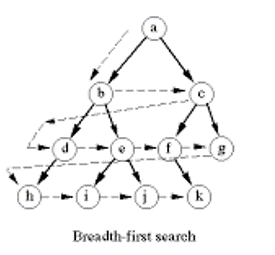
\includegraphics[scale = 0.8]{1.png}
    \caption{BFS algorithm}
    \label{fig:figure1}
\end{figure}

\subsection{Introduction}
We will start by talking about some common sense of the BFS algorithm. We all know that the BFS algorithm will traversal all of the vertices to find the target that we are looking for. If we are doing a BFS in a tree, and we search from the root node, the BFS algorithm can be seen as searching layer by layer from top to bottom. When we deal with a graph, we need to set an initial vertex for the algorithm and the process of the algorithm will spread like a water wave.

So generally speaking, the basic logic of the BFS algorithm is to set up an initial vertex and keep visiting the adjacency until we find the target. 

\subsection{Implementation}
The implementation of the BFS is simple. And since we are dealing with an undirected graph with the same weight for edges. The process becomes easier. Considering the attribute of the BFS itself, every path found by BFS would be exactly the shortest path to the target because every vertex will be immediately added to the queue right after their parents been visited.

we use two functions to implement the kernel goal of the BFS algorithm. 
\begin{itemize}
    \item \verb|connected(vertex)|
    \item \verb|bfs(head, target)|
\end{itemize}

\verb|connect(ver)| will take a vertex as an input. And the output is a list of the adjacency of this vertex. As we mentioned in the last section, the graph that our map mapped to is a list. Also, as we knew, the map of the Snake Game is like a chessboard, that each node has four edges and is vertical to each other. So the mathematical relationship of connected vertices can be described as following:

$a$, $b$ are coordinates of two vertices, when $a$, $b$ can fit the following equations, then they
are connected. $w$ is the length of the map.
\begin{eqnarray}
        a = b - 1 \\
        a = b + 1 \\
        a = b - w \\
        a = b + w 
\end{eqnarray}

Also during the judgment, we need to exclude the walls and the body of the snake, since they 
will be treated as unreachable vertices of the map. This can be easily achieved because we 
store the index of them as attributes in the \verb|solver| class.

\verb|bfs(head, target)| takes the head position of the snake and the target position as 
inputs. And it will return the shortest path from the snake's head to the target. 
To achieve the purpose of BFS, we first need to create a FIFO queue to record the incoming 
vertices. Each time we visited a new vertex, we will add its adjacencies into the queue for 
future visiting. This can be done easily combined with the \verb|connected(ver)|. 
Basically, the process will be going as visiting the vertex whose distance is 1 to head, 
and visited the vertex whose distance is 2 to head and so on. Once we reach the target, 
we will stop the loop.

\subsection{Strategy}

The kernel of the algorithm is to find the shortest path to the food. But it is not enough to
find the shortest path for the snake. Also, we need to tell the snake how it can try to be 
alive, so that snake can get more scores. 

we have the snake to follow three rules for the entire game. The first one is to find the food. 
As long as the snake can reach the food, it will go for it directly. But of course, with the 
game going on, the body of the snake might block the food from the head. This is when the snake
can not reach the food. And here comes the second rule that when the snake can not reach the 
food, it will chase the tail. And of course, there will also be a situation that the snake can
not found the food nor the tail. When we are facing this situation, we'll ask the sanke to move 
randomly and pray for the food can be reached several movements later.

Also, it is obvious that the game is a dynamic process. But the path we found is always based on a map in a certain moment. This means that we may not get the shortest path cause with the movement of snakes body, the connection of each vertex might be updated, then some new path will be created. So we will have the snake find a new path after every movement, though the first path can lead the snake to destination.

\section{A* Approach}
Although BFS algorithm is a very useful approach for a path finding problem, it is not an efficient algorithm. In this section, we use the A* (also known as "A star") path finding algorithm to implement our goals. A* can also find the shortest(or longest) path, but it has a smaller time complexity and a greater space complexity compared to BFS. 

\subsection{Introduction}
Generally speaking, A* algorithm is an advanced version of Dijkstra's algorithm that use a heuristic function to guide its searching path in order to improve the performance. During the searching, instead of just consider the weight of edges like Dijkstra's algorithm, A* also utilize the information of the positions of the vertex. In other word, A* is an informed algorithm. 

If we look at the searching processes of Dijkstra's algorithm and A* , it is easy to tell that A* is much smarter. It behaves like it has already known where the destination vertex is and follows the most possible direction at each action.

A* algorithm can be seen as the combination of Dijkstra's algorithm and Greedy algorithm. We will give a short explanation of them first and finally talk about our implementation of A*. In the following sections, we would use the 2-D square grid as the graph example, which is also the model of our snake game map.

\subsection{Dijkstra's Algorithm \& Greedy Algorithm}

The strategy of Dijkstra's algorithm can be explained as the followings:

\begin{itemize}
    \item Visit the current vertex C, calculate the cost to all it neighbors
    \item Enqueue a neighbor if it is unvisited or the new cost is smaller than old cost
    \item Save the costs into an array disTo, and renew array prev
    \item From pq, select the one that has minimum cost and visit it.
\end{itemize}

Note that the cost is defined as the sum of weights of the edges all along the path, so it tends to visit the neighbors that have smaller weight.

However, in our model, the edges are equal-weighted and every neighbor has equal cost. 
So, as discussed previously, the actual behavior of Dijkstra's algorithm is the same as BFS. 
Following figure shows an example of Dijkstra's searching process.

\begin{figure}[H]
    \centering 
    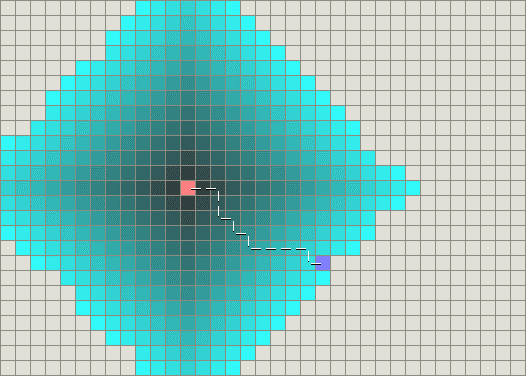
\includegraphics[scale = 0.6]{3.png}
    \caption{Dijkstra's}
\end{figure}

The major advantage of Dijkstra's algorithm is that it always can find the shortest path if it is existed.

The Greedy algorithm follows a very simple strategy: visit the neighbor that has the smallest distance to destination every time. Here we need to use a measurement to define the distance in a 2-D graph. The most common used measurements includes Manhattan distance and Euclidean distance:

\begin{equation*}
    \begin{split}
        &Manhattan Distance = |x_1-x_2|+|y_1-y_2|\\
        &Euclidean Distance = \sqrt{(x_1-x_2)^2+(y_1-y_2)^2}
    \end{split}
\end{equation*}

The implementation is also simple:
\begin{itemize}
    \item Visit current vertex C, mark C visited
    \item Calculate the distances for all its neighbor, visit the one has the smallest distance
\end{itemize}

Also the following figure shows an example of Greedy algorithm searching process.
\begin{figure}[H]
    \centering 
    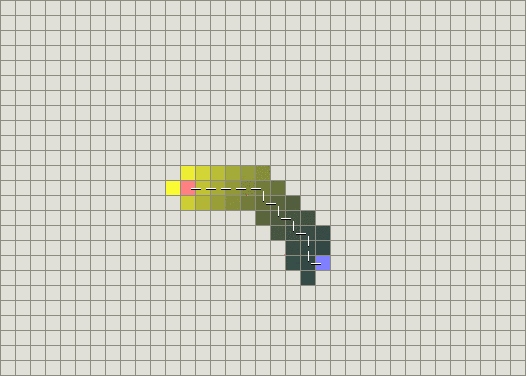
\includegraphics[scale = 0.6]{4.png}
    \caption{Greedy}
\end{figure}

Obviously, Greedy algorithm is very efficient. It acts like it knows where the destination is and use less time to find the shortest path compared to Dijkstra's algorithm.

However, if there is a "wall"(or unreachable vertex) between the starting vertex and ending vertex, Greedy algorithm cannot find the shortest path, the following figure illustrates such situations.

\begin{figure}[H]
    \centering 
    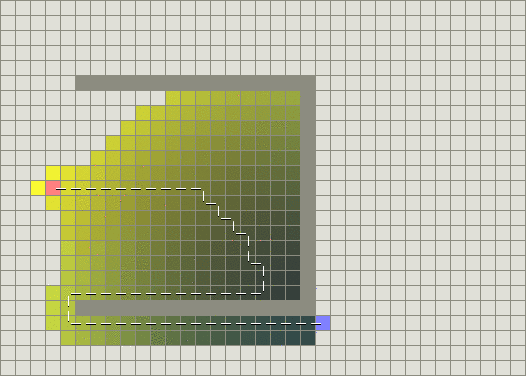
\includegraphics[scale = 0.6]{5.png}
    \caption{Greedy with "wall"}
\end{figure}

\subsection{A* Algorithm \& Implementation}

The initial idea of A* algorithm is to take the Greedy approach as a heuristic information and combine it with Dijkstra's approach. It also use a priority queue for selecting the minimum cost in each iteration. But the cost function is different:

\begin{equation*}
    f(n) = g(n) + h(n;d)
\end{equation*}

Here $f(n)$ is the cost from starting point $s$ to vertex $n$, $g(n)$ is the sum of weights 
along the path from $s$ to $n$, which is the same as Dijkstra's algorithm, and the $h(n;d)$ 
means a heuristic value for $n$ and destination $d$. Usually, $h(n;d)$ is the distance from $n$ 
to $d$, which is the same as Greedy algorithm.

So, why does it work?

\begin{itemize}
    \item Generally, since each "move" has the same cost, A* tends to visit the direction that has less $h(n;d)$.
    \item If there is no impediment, $h(n;d)$ leads the searching path directly toward destination. The Greedy part has greater effect.
    \item If there is a "wall", although $h(n;d)$ first leads to a bad path(more steps) first, but then because of a great $g(n)$, it would cut this path and try another direction. Here the Dijkstra's part has greater effect.
\end{itemize}

\section{Hamiltonian Circle Algorithm}

For above algorithms, they can't finish the game in the situation that the entire map is full of snake body, which means the snake can't eat every food. To solve this problem, we introduce a Hamiltonian Circle and use this into self-playing game to insure the snake can eat every food to the last. Furthermore, we'll put forward advanced Hamiltonian Circle Algorithm adding shortcuts in the naive Hamiltonian Circle Algorithm. There are two mainly contribution in Hamiltonian Circle Algorithm:
\begin{enumerate}
    \item Building the Hamiltonian Circle Algorithm to eat every food generated by random positions in the map. 
    \item Optimizing the Hamiltonian Circle Algorithm by adding shortcuts in early-stage.
\end{enumerate}
    
\subsection{Hamiltonian Circle}
In the mathematical field of graph theory, a Hamiltonian path (or traceable path) is a path in an undirected or directed graph that visits each vertex exactly once. A Hamiltonian cycle (or Hamiltonian circuit) is a Hamiltonian path that is a cycle. In \ref{fig:figure1label}, the red path is Hamiltonian Circle. 
    
\begin{figure}[H]
\centering 
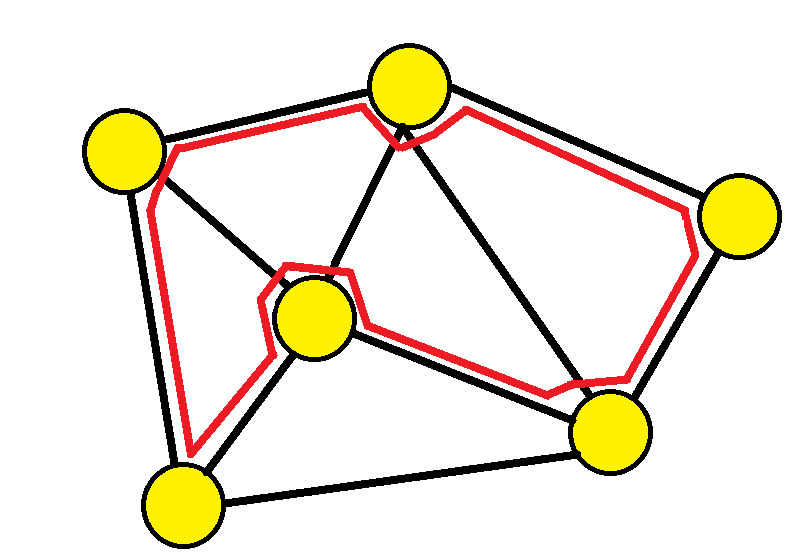
\includegraphics[scale = 0.4]{Hamiltonian.png}
\caption{Hamiltonian Circle.}
\label{fig:figure1label}
\end{figure}

\subsection{Build Hamiltonian Circle}
As we can see, the Hamiltonian Circle can visit every nodes exactly once. As the map in the snake game, the Hamiltonian Circle can visit every single unit exactly once. As Figure \ref{fig:figure2label}, given a initial snake like red arrow including the head direction with the direction of the arrow, we can build a Hamiltonian Circle like yellow path. And then, we can go along the Hamiltonian Circle to eat food successfully until the snake body is full of map. 

\begin{figure}[H]
\centering 
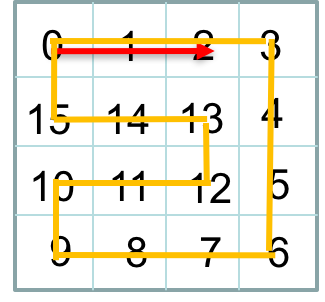
\includegraphics[scale = 0.8]{Picture1.png}
\caption{Hamiltonian Circle in Map.}
\label{fig:figure2label}
\end{figure}

There are two steps to build this yellow Hamiltonian Circle given the initial snake.
\begin{enumerate}
    \item build the shortest path using BFS from head to tail. 
    \item extend the longest path on the foundation of the shortest path above.
\end{enumerate}

First of all, we will build the shortest path using BFS from head to tail. For example, in Figure \ref{fig:figure2label}, putting the node with number 2 into Queue and marking the initial node as distance of 0. Next step, dequeue the node 2 and put the adjacent nodes of number 2 into queue. Marking these adjacent nodes with distance of 1. In the meantime, recording the direction of the parent node. So on and so forth. If we get the tail node in the queue. We can get the path from tail to head by direction of each node's parent nodes. In Figure \ref{fig:figure3label} the third picture is the shortest path using BFS from 2 to 0, head to tail.

Secondly, we will extend the shortest path to a longest path, also known as Hamiltonian Circle in the map. There is a rule in extending the course that if two chosen points are up or down direction, the extending direction will be left or right. For example, in Figure \ref{fig:figure3label}, from picture 3, we can see from head(node2)(1,3), the next points along the shortest path (2,3) has the direction of down from the node2. So we'll extend this two points to the left or right direction. The left direction cannot be extended and the right direction will be chosen. Two points will be extended towards right until to the wall like the path in picture 4. Next, we'll choose next two points (1, 4) and (2,4), but it cannot be extended any direction. Next, we'll choose next two points (2, 4) and (2, 3), the (2, 3) locate in (2, 4) left, so the extending direction is up or down. Down is proper direction. In picture 5 and 6, the result has been shown.

\begin{figure}[H]
\centering 
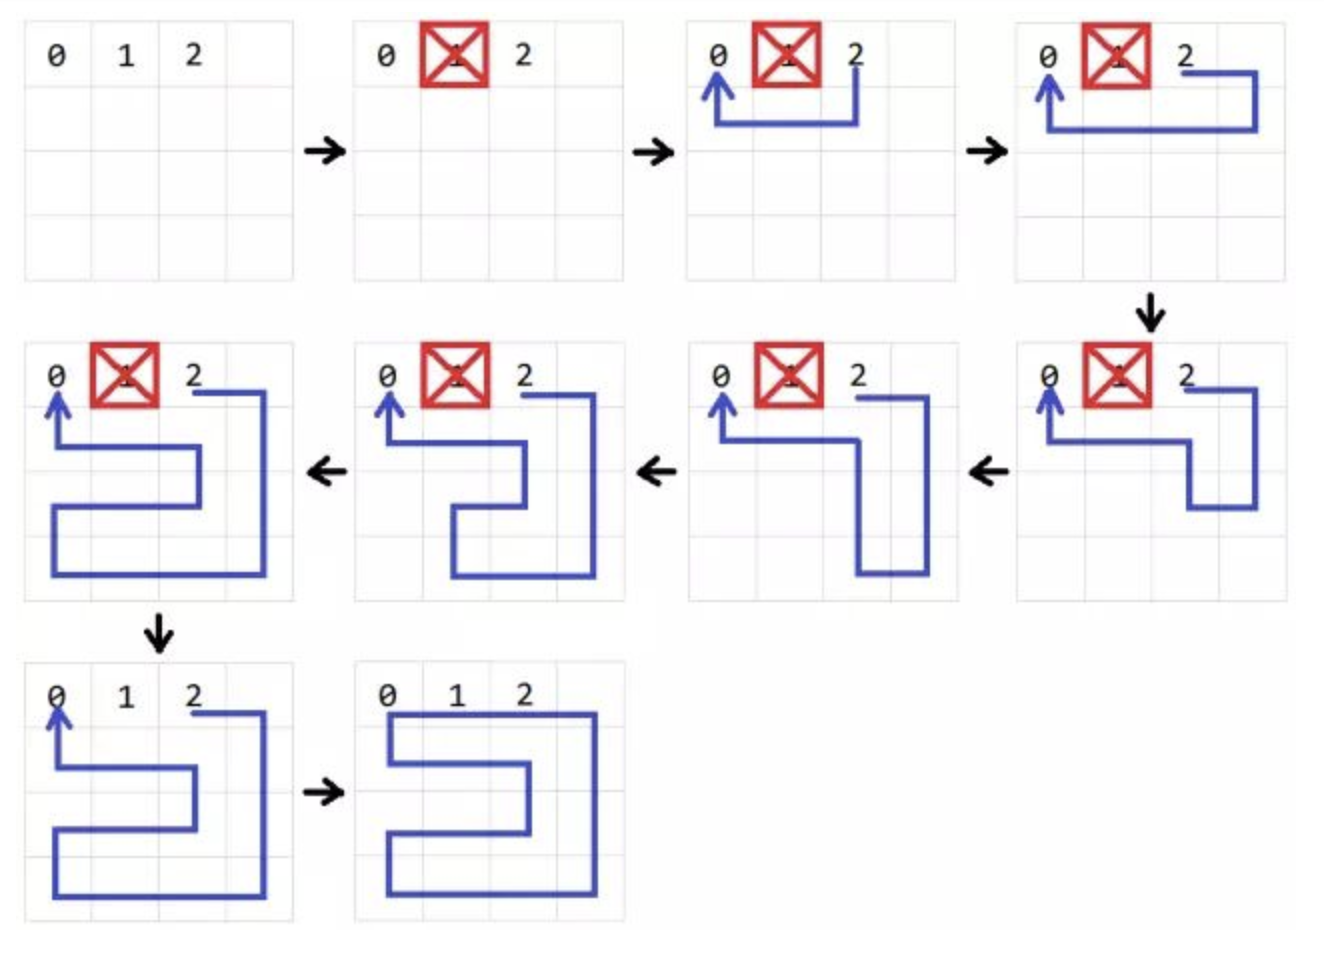
\includegraphics[scale = 0.4]{2.png}
\caption{Build Hamiltonian Circle.}
\label{fig:figure3label}
\end{figure}

Finally, we can get a longest path, which is the Hamiltonian Circle in the map of self-playing snake game.

\subsection{Shortcuts in Hamiltonian Circle Algorithm}

Although Hamiltonian Circle Algorithm can insure the snake eat every food, it need move much steps in total game. Every time the snake need go along the longest path even the food is near the snake head. In this case, we can choose a shortcut in the early-stage to let the total number of movements become smaller. But it needs more time to judge the next direction. That's a trade-off between movement length and direction judgement time. 

The method we use to choose shortcuts is to find the shortest path between current head position and food using BFS and then judge if this direction available. Using BFS to find shortest path is same as the find shortest path between head and tail in the last section. The main point is the second part, how to judge if we choose this next direction. What we do is to find if the next direction is in the body range between head index and tail index. For example, in Figure \ref{fig:figure4label}, the red arrow is current snake. If the next direction judged by using BFS from head to food(not shown in picture) is down, 1, the number in node is  between the number in the head 14 and the tail 4. In this case, we refuse this direction and use Hamiltonian Circle to go next direction 15. If the next direction is up, 1 is not between 14 and 4, we will accept this direction.  

\begin{figure}[H]
\centering 
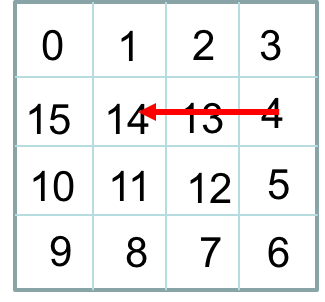
\includegraphics[scale = 0.8]{Picture3.png}
\caption{snake in game.}
\label{fig:figure4label}
\end{figure}

These two algorithm can eat every food until the snake body is full of the map. Two algorithm need build a Hamiltonian Circle when given a initial snake before game starts. Naive Hamiltonian Algorithm doesn't need extra judgement but need more movements length in entire process. Advanced Algorithm including shortcuts need extra judgements but less movements length. That's a trade-off.

\section{Experiments and Analysis}

In this part, we will analyze the results from the performance of each algorithm. We run all the algorithms ten times for different sizes of the map and take the average of each algorithm. We finally decided to take three data for the assessment.
\begin{itemize}
    \item movements per score
    \item runtime(ms) per score
    \item runtime(us) per movement
\end{itemize}

\subsection{Experimental configurations and details}
\begin{itemize}
    \item Processor: AMD Ryzen 3600x
    \item Operation System: Windows 10
    \item Language: Python3
    \item Map Size: 8 10 12 14 16
\end{itemize}


\subsection{Summary}

Before we start to talk about the detailed performance of all algorithms, we can have a whole picture of their performances. The following pictures show how all three snakes directed by algorithms end. We can see that the Hamiltonian algorithms can help the snake to fill up the whole map. Compare to Hamiltonian, BFS and A* show much worse performance on this criterion. Though A* got better performance than BFS, it can only reach half of the map in most times. This shows the foundational differences between Hamiltonian and other algorithms. Hamiltonian focuses more on the surviving problem, which also shows in the analysis of the later performances.

\begin{figure}[H]
    \centering
    \subfigure[BFS]{
        \centering 
        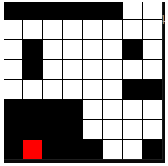
\includegraphics[scale = 0.9]{ana1.png}}
    \subfigure[A*]{
        \centering 
        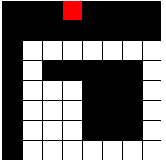
\includegraphics[scale = 0.9]{ana2.png}}
    \subfigure[Hamiltonian]{
        \centering 
        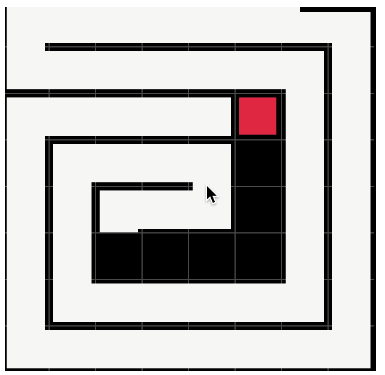
\includegraphics[scale = 0.4]{ana3.png}}

        \caption{Endings of three algorithms}
\end{figure}

\subsection{Performance}
In this section, we will talk about the three criterion mentioned before.
\subsubsection{Movements per score}
This data shows how many movements the snake is going to use to get the food. The reason 
we take this data as one criterion is that one of the purposes we design this project. So 
for each time the snake goes for food, we want the snake to take the shortest path so that 
the program can be more efficient. 

\begin{figure}[H]
    \centering 
    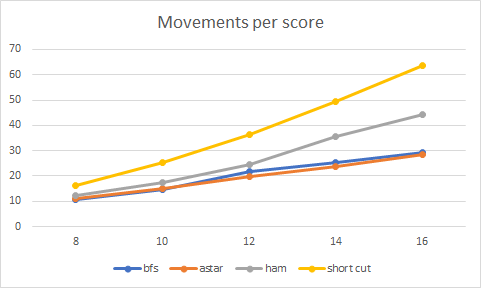
\includegraphics[scale = 0.9]{anay1.png}
    \caption{Movements per score}
\end{figure}

From the figure above, we can see that two Hamiltonian algorithms take more movements to get one 
food, which conforms to what we expected before the implementation. For the Hamiltonian algorithm, 
it takes being alive as the first job. So when it makes a decision on the path to the food, it 
will not always go for the shortest path. Actually, to live longer, the algorithm tends to 
choose the path that is decided according to the Hamiltonian circle, and a Hamiltonian circle will 
always take a longer path so that the snake can live longer. For the A* and BFS, we can see 
that they always take the shorter path to compare to the Hamiltonian circle, cause the strategy 
will urge the snake to go for the shortest path. 

\subsubsection{Runtime(ms) per score}

This criterion is supposed to be relative to the movements it takes to get the food. We get 
this data by dividing the total time by total scores. For A* and BFS, since they take a similar 
strategy and pathfinding algorithm kernel, these two algorithms share a similar performance on 
these two criteria. Also, as we expected, the two algorithms show a little difference. The 
greedy algorithm in A* helps to make a quicker decision. That's where the improvement came from. 

From the figure above, we can see that two Hamiltonian algorithms take more movements to get one food, which conforms to what we expected before the implementation. For the Hamiltonian algorithm, it takes being alive as the first job. So when it makes a decision on the path to the food, it will not always go for the shortest path. Actually, to live longer, the algorithm tends to choose the path that is decided according to the Hamiltonian circle, and a Hamiltonian circle will always take a longer path so that the snake can live longer. For the A* and BFS, we can see that they always take the shorter path to compare to the Hamiltonian circle, because the strategy will urge the snake to go for the shortest path. 

\subsubsection{Runtime(ms) per score}

This criterion is supposed to be relative to the movements it takes to get the food. Runtime can also be viewed as judgement time to next direction. We get this data by dividing the total time by total scores. For A* and BFS, since they take a similar strategy and pathfinding algorithm kernel, these two algorithms share a similar performance on these two criteria. Also, as we expected, the two algorithms show a little difference. The greedy algorithm in A* helps to make a quicker decision. That's where the improvement came from. 

\begin{figure}[H]
    \centering 
    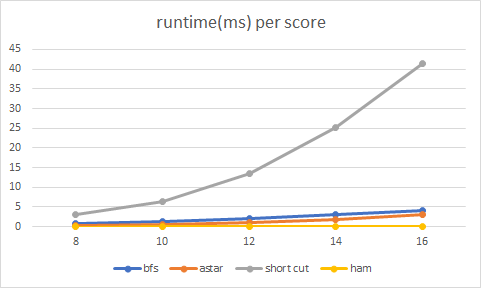
\includegraphics[scale = 0.9]{anay2.png}
    \caption{runtime(ms) per score}
\end{figure}

Meanwhile, the two kinds of Hamiltonian algorithms are extremely different from each other. 
As we mentioned before, the Hamiltonian will only initialize one path that can fill the whole map. 
And then it will go along this path, so it makes no dynamical decision in the whole process, 
that's why its runtime on every score being so small. Otherwise, the Shortcut algorithm will 
dynamically update the path after every movement. 


Meanwhile, the two kinds of Hamiltonian algorithms are extremely different from each other. As we mentioned before, the naive Hamiltonian algorithm will only initialize one path that can fill the whole map. And then it will go along this path, so it makes no dynamical decision in the whole process, that's why its runtime on every score being so small. Otherwise, the Hamiltonian algorithm will dynamically update the path after every movement. 

\subsubsection{Runtime($\mu$s) per movement}



\begin{figure}[H]
    \centering 
    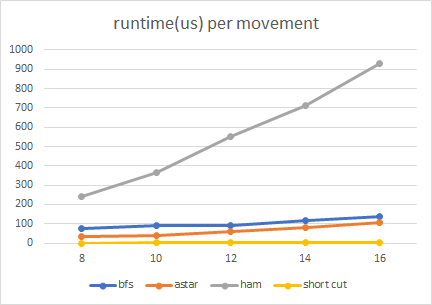
\includegraphics[scale = 0.9]{anay3.png}
    \caption{runtime($\mu$s) per movement}
\end{figure}

This criterion is computed by dividing total runtime by total movements. As we can see, 
this graph shows the same tendency as the last one. And also, the runtime will rise with the 
body of the snake getting longer. That is because as the body getting longer, there will be 
more walls inside the map, which means it will take more movements to get the food. Relatively, 
it will take more time for the algorithm to find the path. There is only one exception, 
the Hamiltonian. Because this algorithm only focuses on the initial path, and will not dynamically 
update this path.

\section{Conclusion}

From above experiments, if we view movement length as performance in which less movements is better:

      $$BFS \approx A star < Hamiltonian\ shortcut < Hamiltonian$$
     
if we view extent of alive time (eat more food) as performance in which more score is better:
       
       $$Hamiltonian\ shortcut = Hamiltonian > Astar > BFS$$
       
if we view the runtime (judgement time) per movement as performance, less is better:
      $$Hamiltonian > A star > BFS > Hamiltonian\ shortcut$$
      
That's a trade-off between movements length and alive score. Depends on which performance we need. Beyond that, if we need less runtime (judgement time), Astar or Hamiltonian is better.

\section{Contribution}

Yang Sui: Hamilton Algorithm, Snake Game Implementation, Analysis\\
Jin Xu: A* Approach, Snake Game Implementation, Analysis\\
Runlin Hou: BFS Approach, Analysis

\end{document}